%
% starship.tex -- schnellste Bahn in eine Umlaufbahn
%
% (c) 2021 Prof Dr Andreas Müller, OST Ostschweizer Fachhochschule
%
\bgroup
\def\zykloid{
 ({97.0000}:\R)
 -- ({97.0000}:{\R+0.0005})
 -- ({96.9998}:{\R+0.0020})
 -- ({96.9994}:{\R+0.0044})
 -- ({96.9985}:{\R+0.0079})
 -- ({96.9971}:{\R+0.0123})
 -- ({96.9950}:{\R+0.0177})
 -- ({96.9921}:{\R+0.0241})
 -- ({96.9882}:{\R+0.0314})
 -- ({96.9833}:{\R+0.0397})
 -- ({96.9771}:{\R+0.0489})
 -- ({96.9695}:{\R+0.0591})
 -- ({96.9605}:{\R+0.0702})
 -- ({96.9498}:{\R+0.0822})
 -- ({96.9374}:{\R+0.0952})
 -- ({96.9231}:{\R+0.1090})
 -- ({96.9069}:{\R+0.1237})
 -- ({96.8885}:{\R+0.1393})
 -- ({96.8678}:{\R+0.1557})
 -- ({96.8448}:{\R+0.1729})
 -- ({96.8194}:{\R+0.1910})
 -- ({96.7913}:{\R+0.2098})
 -- ({96.7606}:{\R+0.2295})
 -- ({96.7270}:{\R+0.2499})
 -- ({96.6906}:{\R+0.2710})
 -- ({96.6511}:{\R+0.2929})
 -- ({96.6085}:{\R+0.3155})
 -- ({96.5627}:{\R+0.3387})
 -- ({96.5137}:{\R+0.3626})
 -- ({96.4612}:{\R+0.3871})
 -- ({96.4053}:{\R+0.4122})
 -- ({96.3458}:{\R+0.4379})
 -- ({96.2826}:{\R+0.4642})
 -- ({96.2158}:{\R+0.4910})
 -- ({96.1451}:{\R+0.5182})
 -- ({96.0706}:{\R+0.5460})
 -- ({95.9922}:{\R+0.5742})
 -- ({95.9098}:{\R+0.6029})
 -- ({95.8234}:{\R+0.6319})
 -- ({95.7329}:{\R+0.6613})
 -- ({95.6382}:{\R+0.6910})
 -- ({95.5394}:{\R+0.7210})
 -- ({95.4363}:{\R+0.7513})
 -- ({95.3290}:{\R+0.7819})
 -- ({95.2174}:{\R+0.8126})
 -- ({95.1015}:{\R+0.8436})
 -- ({94.9812}:{\R+0.8747})
 -- ({94.8566}:{\R+0.9059})
 -- ({94.7275}:{\R+0.9372})
 -- ({94.5941}:{\R+0.9686})
 -- ({94.4563}:{\R+1.0000})
 -- ({94.3141}:{\R+1.0314})
 -- ({94.1675}:{\R+1.0628})
 -- ({94.0166}:{\R+1.0941})
 -- ({93.8612}:{\R+1.1253})
 -- ({93.7015}:{\R+1.1564})
 -- ({93.5374}:{\R+1.1874})
 -- ({93.3690}:{\R+1.2181})
 -- ({93.1963}:{\R+1.2487})
 -- ({93.0194}:{\R+1.2790})
 -- ({92.8382}:{\R+1.3090})
 -- ({92.6529}:{\R+1.3387})
 -- ({92.4634}:{\R+1.3681})
 -- ({92.2698}:{\R+1.3971})
 -- ({92.0722}:{\R+1.4258})
 -- ({91.8706}:{\R+1.4540})
 -- ({91.6651}:{\R+1.4818})
 -- ({91.4558}:{\R+1.5090})
 -- ({91.2426}:{\R+1.5358})
 -- ({91.0258}:{\R+1.5621})
 -- ({90.8053}:{\R+1.5878})
 -- ({90.5812}:{\R+1.6129})
 -- ({90.3537}:{\R+1.6374})
 -- ({90.1227}:{\R+1.6613})
 -- ({89.8885}:{\R+1.6845})
 -- ({89.6511}:{\R+1.7071})
 -- ({89.4106}:{\R+1.7290})
 -- ({89.1670}:{\R+1.7501})
 -- ({88.9206}:{\R+1.7705})
 -- ({88.6713}:{\R+1.7902})
 -- ({88.4194}:{\R+1.8090})
 -- ({88.1648}:{\R+1.8271})
 -- ({87.9078}:{\R+1.8443})
 -- ({87.6485}:{\R+1.8607})
 -- ({87.3869}:{\R+1.8763})
 -- ({87.1231}:{\R+1.8910})
 -- ({86.8574}:{\R+1.9048})
 -- ({86.5898}:{\R+1.9178})
 -- ({86.3205}:{\R+1.9298})
 -- ({86.0495}:{\R+1.9409})
 -- ({85.7771}:{\R+1.9511})
 -- ({85.5033}:{\R+1.9603})
 -- ({85.2282}:{\R+1.9686})
 -- ({84.9521}:{\R+1.9759})
 -- ({84.6750}:{\R+1.9823})
 -- ({84.3971}:{\R+1.9877})
 -- ({84.1185}:{\R+1.9921})
 -- ({83.8394}:{\R+1.9956})
 -- ({83.5598}:{\R+1.9980})
 -- ({83.2800}:{\R+1.9995})
}

\begin{frame}[t]
\setlength{\abovedisplayskip}{5pt}
\setlength{\belowdisplayskip}{5pt}
\frametitle{Der billigste Weg in eine Umlaufbahn}
\vspace{-15pt}
\begin{center}
\def\a{10}
\def\s{12}
\def\d{1.16}
\pgfmathparse{6/sin(\a)}
\xdef\R{\pgfmathresult}
\begin{tikzpicture}[>=latex]
\begin{scope}
\clip (-6.3,{\R*cos(\a)-1}) rectangle ++(12.6,3.6);
\foreach \y in {2,1.9,...,0}{
	\pgfmathparse{((2-\y)*(2-\y))/4}
	\xdef\o{\pgfmathresult}
	\fill[color=blue!20,opacity=\o]
		(0,0) -- ({90-\a}:{\R+\y}) arc ({90-\a}:{90+\a}:{\R+\y}) -- cycle;
}
\fill[color=brown]
	({90-\a}:{\R-1.05})
	-- ({90-\a}:\R) arc ({90-\a}:{90+\a}:\R)
	-- (90+\a:{\R-1.05})
	-- cycle;
\uncover<2->{
\draw[line width=2pt,color=red!20] (0,0) circle[radius={\R+2}];
}
\uncover<3->{
\draw[line width=3pt,color=red] (70:\R+2) arc (70:{90-6.2}:\R+2);
}
\end{scope}
\only<1-3>{
\node at ({90+7}:{\R+0.9}) [rotate=7]
{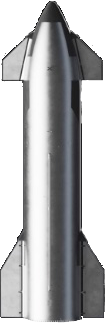
\includegraphics[width=0.6cm]{../slides/0/starship.png}};
}
\only<4->{
\node at ({90-7-\d}:{\R+2}) [rotate={-97-\d}]
{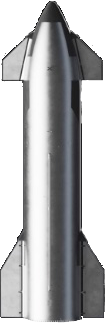
\includegraphics[width=0.6cm]{../slides/0/starship.png}};
}
\begin{scope}
\clip (-6.2,{\R*cos(\a)}) rectangle ++(12.4,3.6);
\uncover<3->{
\draw[line width=3pt,color=red] \zykloid;
}
\end{scope}
\end{tikzpicture}
\end{center}
\vspace*{-16pt}
\begin{columns}[t,onlytextwidth]
\begin{column}{0.48\textwidth}
\begin{block}{Ziel}
\begin{itemize}
\item<2-> Treibstoffbedarf minimieren
\item<5-> Strukturelle Integrität erhalten
\end{itemize}
\end{block}
\end{column}
\begin{column}{0.48\textwidth}
\end{column}
\end{columns}
\end{frame}
\egroup
